% ---------------------------------------------------------------------------
%  Suggestion: place in Section 3, just before Proposition 5, with
%  \ref{fig:landscape} in the text.
%  Generated from the certificate by gen_tikz.py; edit that, not this.
% ---------------------------------------------------------------------------
\begin{figure}[H]
\centering
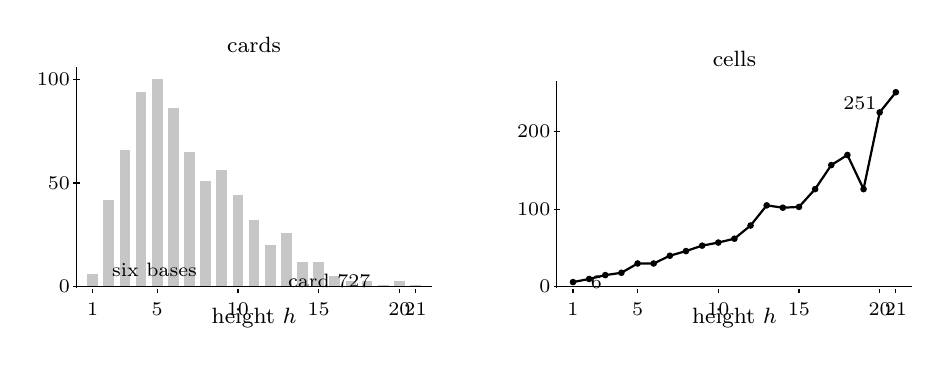
\begin{tikzpicture}[x=2.05mm,y=1pt,font=\small]
\begin{scope}
\fill[gray!45] (0.67,0) rectangle (1.33,4.50);
\fill[gray!45] (1.67,0) rectangle (2.33,31.50);
\fill[gray!45] (2.67,0) rectangle (3.33,49.50);
\fill[gray!45] (3.67,0) rectangle (4.33,70.50);
\fill[gray!45] (4.67,0) rectangle (5.33,75.00);
\fill[gray!45] (5.67,0) rectangle (6.33,64.50);
\fill[gray!45] (6.67,0) rectangle (7.33,48.75);
\fill[gray!45] (7.67,0) rectangle (8.33,38.25);
\fill[gray!45] (8.67,0) rectangle (9.33,42.00);
\fill[gray!45] (9.67,0) rectangle (10.33,33.00);
\fill[gray!45] (10.67,0) rectangle (11.33,24.00);
\fill[gray!45] (11.67,0) rectangle (12.33,15.00);
\fill[gray!45] (12.67,0) rectangle (13.33,19.50);
\fill[gray!45] (13.67,0) rectangle (14.33,9.00);
\fill[gray!45] (14.67,0) rectangle (15.33,9.00);
\fill[gray!45] (15.67,0) rectangle (16.33,3.75);
\fill[gray!45] (16.67,0) rectangle (17.33,2.25);
\fill[gray!45] (17.67,0) rectangle (18.33,2.25);
\fill[gray!45] (18.67,0) rectangle (19.33,0.75);
\fill[gray!45] (19.67,0) rectangle (20.33,2.25);
\fill[gray!45] (20.67,0) rectangle (21.33,0.75);
\draw (-.1,0)--(22,0);
\draw (0,-.5)--(0,79.50);
\draw (-.2,0.00)--(.2,0.00) node[left,font=\scriptsize] {0};
\draw (-.2,37.50)--(.2,37.50) node[left,font=\scriptsize] {50};
\draw (-.2,75.00)--(.2,75.00) node[left,font=\scriptsize] {100};
\draw (1.0,-.8)--(1.0,-2.2) node[below,font=\scriptsize] {1};
\draw (5.0,-.8)--(5.0,-2.2) node[below,font=\scriptsize] {5};
\draw (10.0,-.8)--(10.0,-2.2) node[below,font=\scriptsize] {10};
\draw (15.0,-.8)--(15.0,-2.2) node[below,font=\scriptsize] {15};
\draw (20.0,-.8)--(20.0,-2.2) node[below,font=\scriptsize] {20};
\draw (21.0,-.8)--(21.0,-2.2) node[below,font=\scriptsize] {21};
\node[below,font=\footnotesize] at (11,-4.2) {height $h$};
\node[font=\footnotesize] at (11,87.50) {cards};
\node[font=\scriptsize,anchor=west] at (1.6,6.00) {six bases};
\node[font=\scriptsize,anchor=west] at (12.5,2.25) {card $727$};
\end{scope}
\begin{scope}[xshift=6.1cm]
\draw[thick] (1.0,1.68)--(2.0,2.80)--(3.0,4.20)--(4.0,5.04)--(5.0,8.40)--(6.0,8.40)--(7.0,11.20)--(8.0,12.88)--(9.0,14.84)--(10.0,15.96)--(11.0,17.36)--(12.0,22.12)--(13.0,29.40)--(14.0,28.56)--(15.0,28.84)--(16.0,35.28)--(17.0,43.96)--(18.0,47.60)--(19.0,35.28)--(20.0,63.00)--(21.0,70.28);
\fill (1.0,1.68) circle (1.2pt);
\fill (2.0,2.80) circle (1.2pt);
\fill (3.0,4.20) circle (1.2pt);
\fill (4.0,5.04) circle (1.2pt);
\fill (5.0,8.40) circle (1.2pt);
\fill (6.0,8.40) circle (1.2pt);
\fill (7.0,11.20) circle (1.2pt);
\fill (8.0,12.88) circle (1.2pt);
\fill (9.0,14.84) circle (1.2pt);
\fill (10.0,15.96) circle (1.2pt);
\fill (11.0,17.36) circle (1.2pt);
\fill (12.0,22.12) circle (1.2pt);
\fill (13.0,29.40) circle (1.2pt);
\fill (14.0,28.56) circle (1.2pt);
\fill (15.0,28.84) circle (1.2pt);
\fill (16.0,35.28) circle (1.2pt);
\fill (17.0,43.96) circle (1.2pt);
\fill (18.0,47.60) circle (1.2pt);
\fill (19.0,35.28) circle (1.2pt);
\fill (20.0,63.00) circle (1.2pt);
\fill (21.0,70.28) circle (1.2pt);
\draw (-.1,0)--(22,0);
\draw (0,-.5)--(0,74.20);
\draw (-.2,0.00)--(.2,0.00) node[left,font=\scriptsize] {0};
\draw (-.2,28.00)--(.2,28.00) node[left,font=\scriptsize] {100};
\draw (-.2,56.00)--(.2,56.00) node[left,font=\scriptsize] {200};
\draw (1.0,-.8)--(1.0,-2.2) node[below,font=\scriptsize] {1};
\draw (5.0,-.8)--(5.0,-2.2) node[below,font=\scriptsize] {5};
\draw (10.0,-.8)--(10.0,-2.2) node[below,font=\scriptsize] {10};
\draw (15.0,-.8)--(15.0,-2.2) node[below,font=\scriptsize] {15};
\draw (20.0,-.8)--(20.0,-2.2) node[below,font=\scriptsize] {20};
\draw (21.0,-.8)--(21.0,-2.2) node[below,font=\scriptsize] {21};
\node[below,font=\footnotesize] at (11,-4.2) {height $h$};
\node[font=\footnotesize] at (11,82.20) {cells};
\node[font=\scriptsize,anchor=west] at (1.5,1.68) {$6$};
\node[font=\scriptsize,anchor=east] at (20.4,66.28) {$251$};
\end{scope}
\end{tikzpicture}
\caption{The certificate as a whole. Left, the number of cards at each height: a
pyramid from the six one-hole copies to the single card $727$. Right, the largest
envelope at each height. The two trends are the reason the construction works:
the higher a card reaches, the more cells it must keep free of Breaker
($251$ at the top), while the required sets move the other way and end empty.}
\label{fig:landscape}
\end{figure}
